\documentclass[main]{subfiles}


\begin{document}
\newpage
\section{Prediction Errors During Perception And Learning}
\subsection{Motivation}
There are many theories and principles about the brain such as free-energy principle, predictive coding theory and theories about error back-propagation in the brain. These different approaches attempt to explain the structure and function of the brain from a probabilistic inference perspective focusing on error propagation. 

In this chapter, we, as well, consider prediction and perceptual categorization as an inference problem that is solved by the brain\footnote{Friston $&$ Kiebal. Predictive coding under the free-energy principle. \textit{Philosophical Transactions of The Royal Society B Biological Sciences}· June 2009.}. Under our view, in this chapter, the brain models the world as a hierarchy of dynamic systems. One key difference between this view and what we have learnt in the previous chapter on variational inference lies in the distinction between discriminative and generative models\footnote{https://www.cs.toronto.edu/~duvenaud/courses/csc2541/index.html}.


\subsubsection{Discriminative Vs Generative Models}


\paragraph{Discriminative models}
In Chapter 5, we were concerned with regression/classification tasks where we were interested in obtaining the conditional distribution \textbf{$p(t|\bm{x},\bm{w})$. }
\noindent
Models falling into this category are well-suited for supervised-learning problems. There is a teacher providing the targets which helps us learn the mapping from inputs to targets. 

\noindent
But what if, we don't have the targets, i.e no labelled data is at our disposal? Or what if we don't have a clear view of what we want to discriminate? Then comes the importance of generative models.

\paragraph{Generative models}
This type of modelling refers to building a \textbf{model of the data}, $p(\bm{x})$ from which we can sample. But what are our practical reasons for doing so?

\begin{itemize}
    \item [--] \textbf{Data efficiency}: explain the world using less data points. 
    \item [--] Better \textbf{understanding}: one key feature of generative models is interpretability. Generative models assume, as we will see, that the data is generated from some low-dimensional latent factors or variables to which we can assign meaning. In other words, we can associate each latent variable to a cause, something that would allow us to interpret a phenomenon.
    \item [--] \textbf{Model checking} by sampling: Regression and classification models are usually complex. It is often hard to check what these models have captured from the data and what did they miss. One advantage of generative modelling is that it allows us to perform a sanity-check. Since we know the probability distribution generating the data, we can easily sample from it and compare the sampled data to the real data to see if anything is missing. This goes back to famous quote by Richard Feynman, 1988: "What I cannot create, I do not understand."
    \item [--] \textbf{Compression}:
    in generative modelling, we seek to explain the data (ex. some sensory input $\bm{x}$) using with a low-dimensional latent variables ($\bm{h}$). We have therefore compressed the information (from complex, high-dimensional data $\rightarrow$ low-dimensional, simpler description), which is at the core of Chaitin's 2007 "Comprehension is compression". \hl{A model is better is it explains more with less.}
    \item [--] \hl{Online classification: novel content?}
\end{itemize}

\subsubsection{Recap Bayesian inference}
In the previous lecture, we formulated learning as a Bayesian inference problem. We started by defining a model using a prior on the weights (modelled as random variables following a probability distribution) and a likelihood function (which captures how likely is it that the data we see is generated under our model), then tried to update, using Bayes' rule, the weight distribution after seeing the data, i.e:

\paragraph{Recipe for Bayesian inference}\mbox{}\\


\fbox{%
    \parbox{\textwidth}{%
    \begin{enumerate}
        \item \textbf{Define the model} 
            \begin{itemize}
                \item [--] $p(\bm{w})$: could be a pre-trained model or any other prior on the weights.
                \item [--] $p(\bm{t}|\bm{x},\bm{w})$ referred to as \textbf{forward probability}. Note that for inference we assume $\bm{w}$ fixed and we infer $\bm{t}$ from $\bm{x}$. In the machine learning view, this is a "noisy" neural network.\newline
                $f_{NN}(\bm{x}, \bm{w}) + noise$
            \end{itemize}
            
            \begin{figure}[H]
            	\centering
            	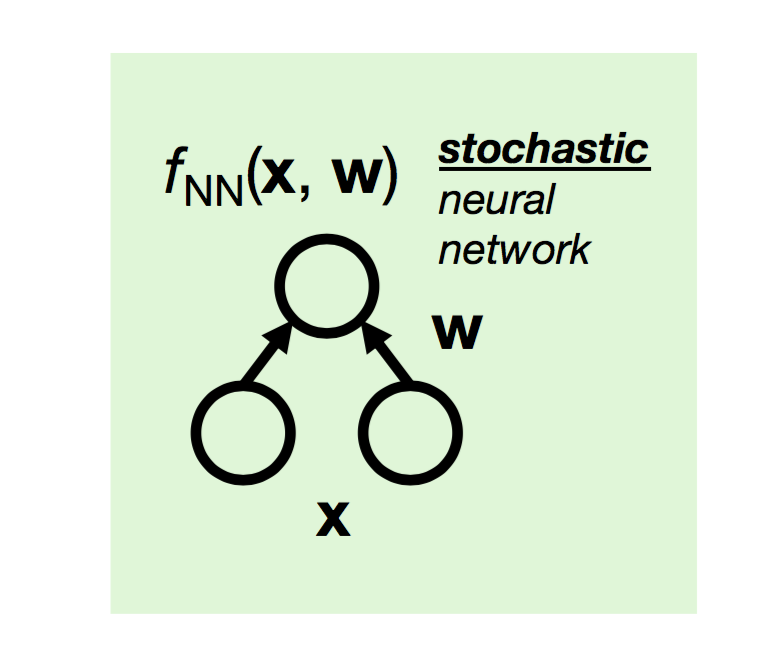
\includegraphics[width=0.4\linewidth]{06_PredictionErrorsDuringPerceptionAndLearning/figures/inference_NN.png}
            	\caption{Computing the forward probability using a stochastic neural network.} 
            	\label{fig:NN_inference}
            \end{figure}
            
        \item \textbf{Learn/ Update model}: using Bayes' rule; where $D = \big\{\bm{x}^{(n)}, \bm{t}^{(n)}\} ^N_{n=1} $
            \begin{equation}
                p(\bm{w}|D) = \frac{p(\bm{t}|\bm{x}, \bm{w}). p(\bm{w})}{\int_\Omega p(\bm{t}|\bm{x}, \bm{w}). p(\bm{w}) d\bm{w}}
            \end{equation}
            referred to as \textbf{inverse probability} because we are inverting the model.
    \end{enumerate}
    }}
\paragraph{Some comments before diving deeper}
\begin{itemize}
    \item [--] In the previous chapter, we relied on the target $\bm{t}$. But we might ask, does the brain \textbf{always} rely on a teacher signal/ target?
    \item [--] In this chapter we are building a model of the data. Such general knowledge of the world can help us know \textbf{"what to expect"}, which is important for decision-making agencies. Furthermore, a general knowledge can allow us to build our own labels on the fly; we can hence start to classify things on the fly. \hl{more details...}
    \item [--] In Chapter 5, we had to worry about the marginal probability $p(\bm{x})$ because we wanted apply Bayes' rule. In this chapter, \textbf{we are not fully Bayesian} and will use a frequentist approach as a shortcut. \hl{(in inference MAP)}
    \item [--] Why are we particularly concerned with perception? Simply because it is beleived that the brain learns a generative model for its stream of sensory data. Put differently, our brain learns a model of how sensory data are generated which can be  thought of as "a particular type of probabilistic model that captures cause and effect"\footnote{Nice blog post: http://boxandarrowbrain.com/2018/02/06/generative-models-in-perception/}. Perception is then equated to inverting the generic model, reasoning about causes after observing the effects.
\end{itemize}

\subsection{Hierarchical Gaussian Models (HGM)}
We focus on a particular class of generative models; we consider models that can be structured as a hierarchy of latent variables, $\bm{h}$ comprising of N layers:

\begin{equation}
    \boxed{
    p(\bm{x},\bm{h_1}\dots, \bm{h_N}) = p(\bm{x}|\bm{h_1}).p(\bm{h_1}|\bm{h_2})\dots .p(\bm{h_{N-1}}|\bm{h_N}). p(\bm{h_N})}
    \label{eq:joint_density}
\end{equation}

    \begin{figure}[H]
            	\centering
            	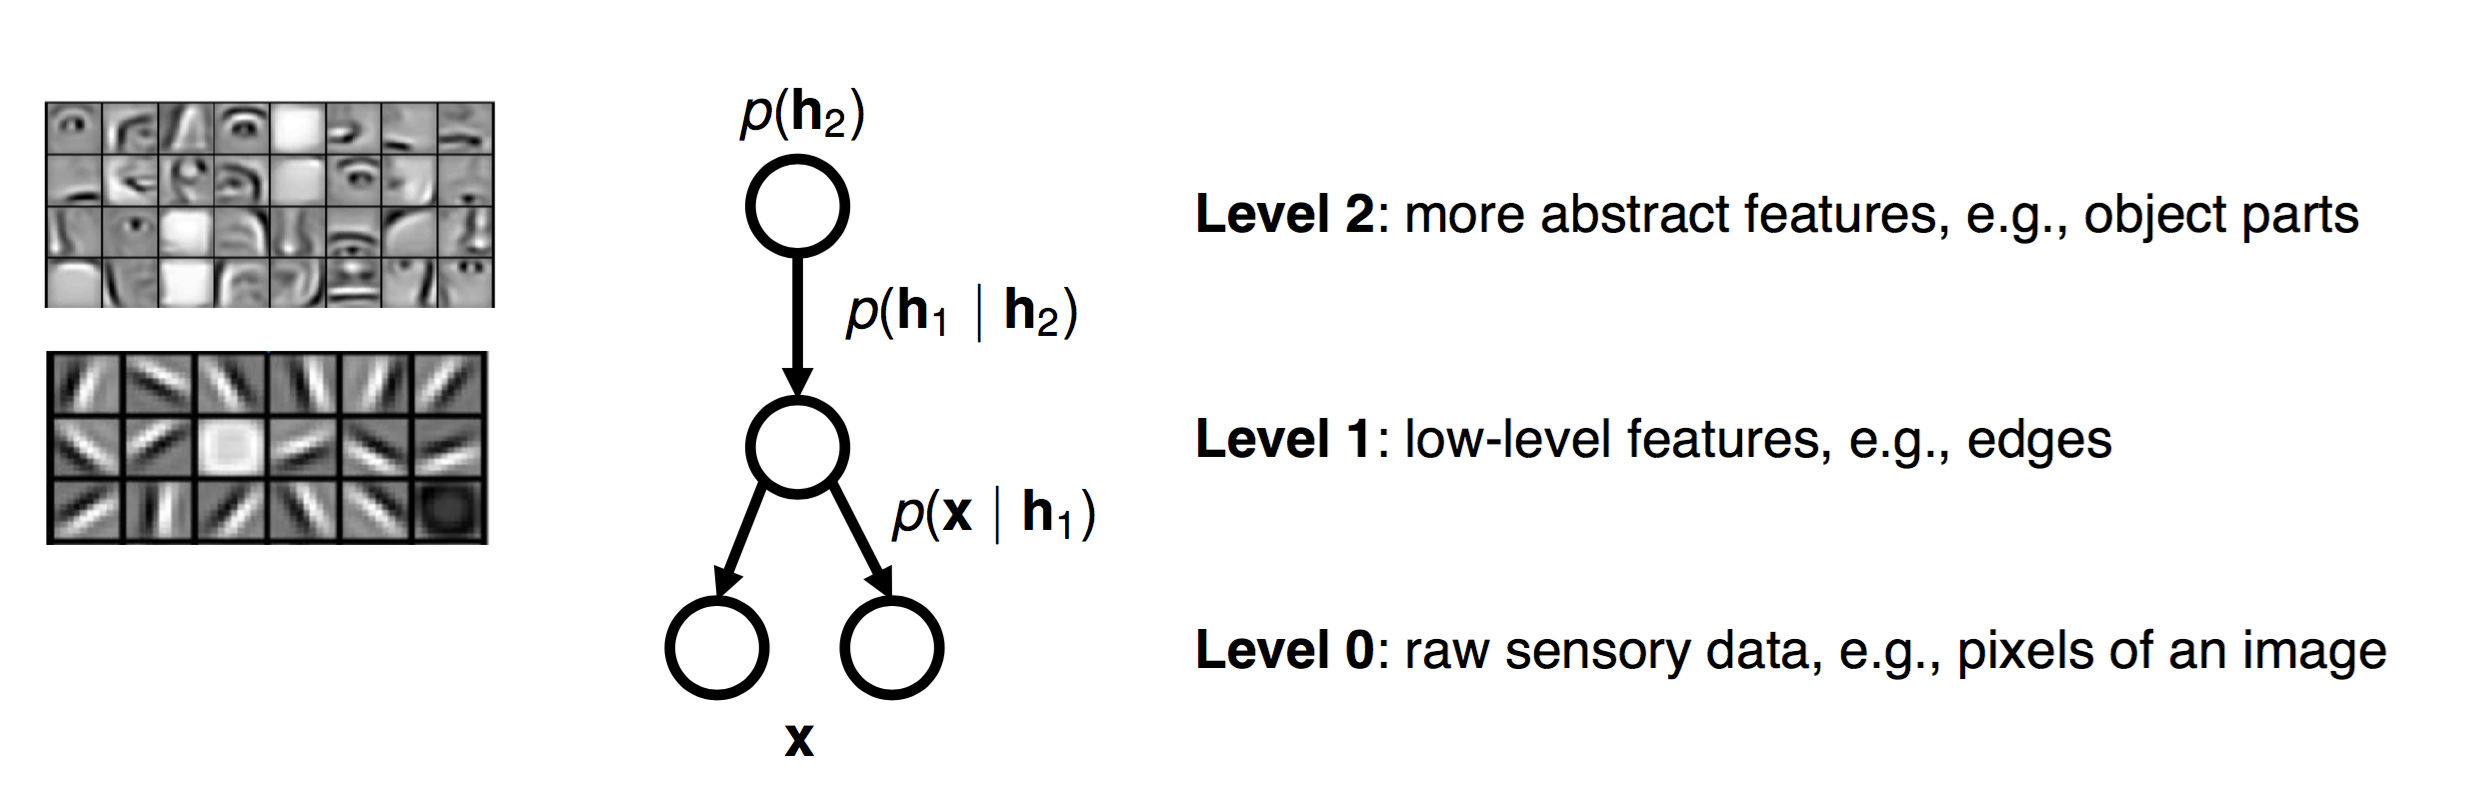
\includegraphics[width=1\linewidth]{06_PredictionErrorsDuringPerceptionAndLearning/figures/hierarchical_models.png}
            	\caption{Example of generative model with a hierarchical structure comprised of 3 layers.} 
            	\label{fig:hierar_model}
    \end{figure}

\subsubsection{Perception as probabilistic inference}
As explained earlier, perception can be seen as finding causes given that we have observed the effects.\hl{elaborate using an example from blog post...}

In such context and following the same approach from Chapter 5, we perform inference on the latent variables instead of the targets $\bm{t}$ using Bayes' rule to obtain a distribution over our latent variable, given an observed sensory input $\bm{x}$.
\fbox{%
    \parbox{\textwidth}{%
    \begin{enumerate}
        \item \textbf{Define the model over $\bm{h}$} 
                \begin{itemize}
                    \item [--] $p(\bm{h})$
                    \item [--] $p(\bm{x}|\bm{h})$ referred to as \textbf{forward probability}. Note that for inference we assume $\bm{h}$ fixed and we infer $\bm{x}$ from $\bm{h}$.
                \end{itemize}
                
        \item \textbf{Perceive} = invert the model
                \begin{equation}
                    p(\bm{h}|\bm{x}) = \frac{p(\bm{x}|\bm{h}). p(\bm{h})}{\int_H p(\bm{x}|\bm{h}). p(\bm{h}) d\bm{h}}
                    \label{eq:bayes_generative_model}
                \end{equation}
                referred to as \textbf{inverse probability}.
     
    \end{enumerate}
}}


\subsubsection{Model Assumptions}
\begin{itemize}
    \item We assume each conditional probability distribution $p(\bm{h}_i|\bm{h}_{i+1})$ is Gaussian with mean dependent on the higher order variable $\bm{h_{i+1}}$ and covariance matrix $\Sigma_i$. Using the convention that the first layer later variable corresponds to the input, i.e. $\bm{h_0} = \bm{x}$:
        \begin{equation}
            p(\bm{h_i}|\bm{h_{i+1}}) \sim N(\bm{h_i}; \mu_i(\bm{h_{i+1}}), \Sigma_i)
        \end{equation}
        
    \item Assume a Gaussian top-level prior, \textbf{layer N} (and will briefly discuss a Laplacian prior)
       \begin{equation}
            p(\bm{h_N}) \sim N(\bm{h_N}; \mu_N, \Sigma_N)
        \end{equation}
    \item Note that the joint distribution $p(\bm{x},\bm{h_1}\dots, \bm{h_N})$ is in general not Gaussian for this model (only true for the special case of linear $\bm{\mu_i}$)
    
    \item We link two consecutive layers and introduce non-linearity, $\phi$, with the following parameterization of the conditional mean:
        \begin{equation}
            \mu_i(\bm{h_{i+1}}) = \bm{w_{i}}. \phi(\bm{h_{i+1}}) + \bm{b_i}
        \end{equation}
        where $\bm{b_i}$ is the vector of biases
    
    \item From the previous assumptions, we can denote our model's parameters as $\bm{\Theta}$:
        \begin{equation}
            \begin{split}
                 \Theta &= \big\{ \bm{W_i}, \bm{b_i}, \Sigma_i\} \\
                        &= \{ \mu_N, \Sigma_N\} 
            \end{split}
        \end{equation}
    \item \textbf{Note}: we will include the bias vector as an additional weight column and set all covariance matrices $\Simga_i$ to identity matrix $I$:
        \begin{equation}
            I= diag(1,1 \dots , 1)
        \end{equation}
        
\end{itemize}

\subsubsection{Inference under the Hierarchical Generative Model}
Inference is about inversion of the internal states of the models.\\

\noindent
\textbf{Note that to perform inference we assume the model parameters $\Theta$ to be fixed.}\\

\noindent
In order to invert the internal states, we need to:
\begin{enumerate}
    \item Find $p(\bm{h}|\bm{x};\Theta)$ using Bayes' rule in eq. \ref{eq:bayes_generative_model}.
    \item Get a point estimate for the latent variable $\bm{h}$ using \textbf{a maximum a posteriori (MAP)} criterion. In other words, we try to find an optimal $\bm{h}$ that maximizes the posterior distribution $p(\bm{h}|\bm{x};\Theta)$ (this explains why we are not fully Bayesian).
        \begin{figure}[H]
            	\centering
            	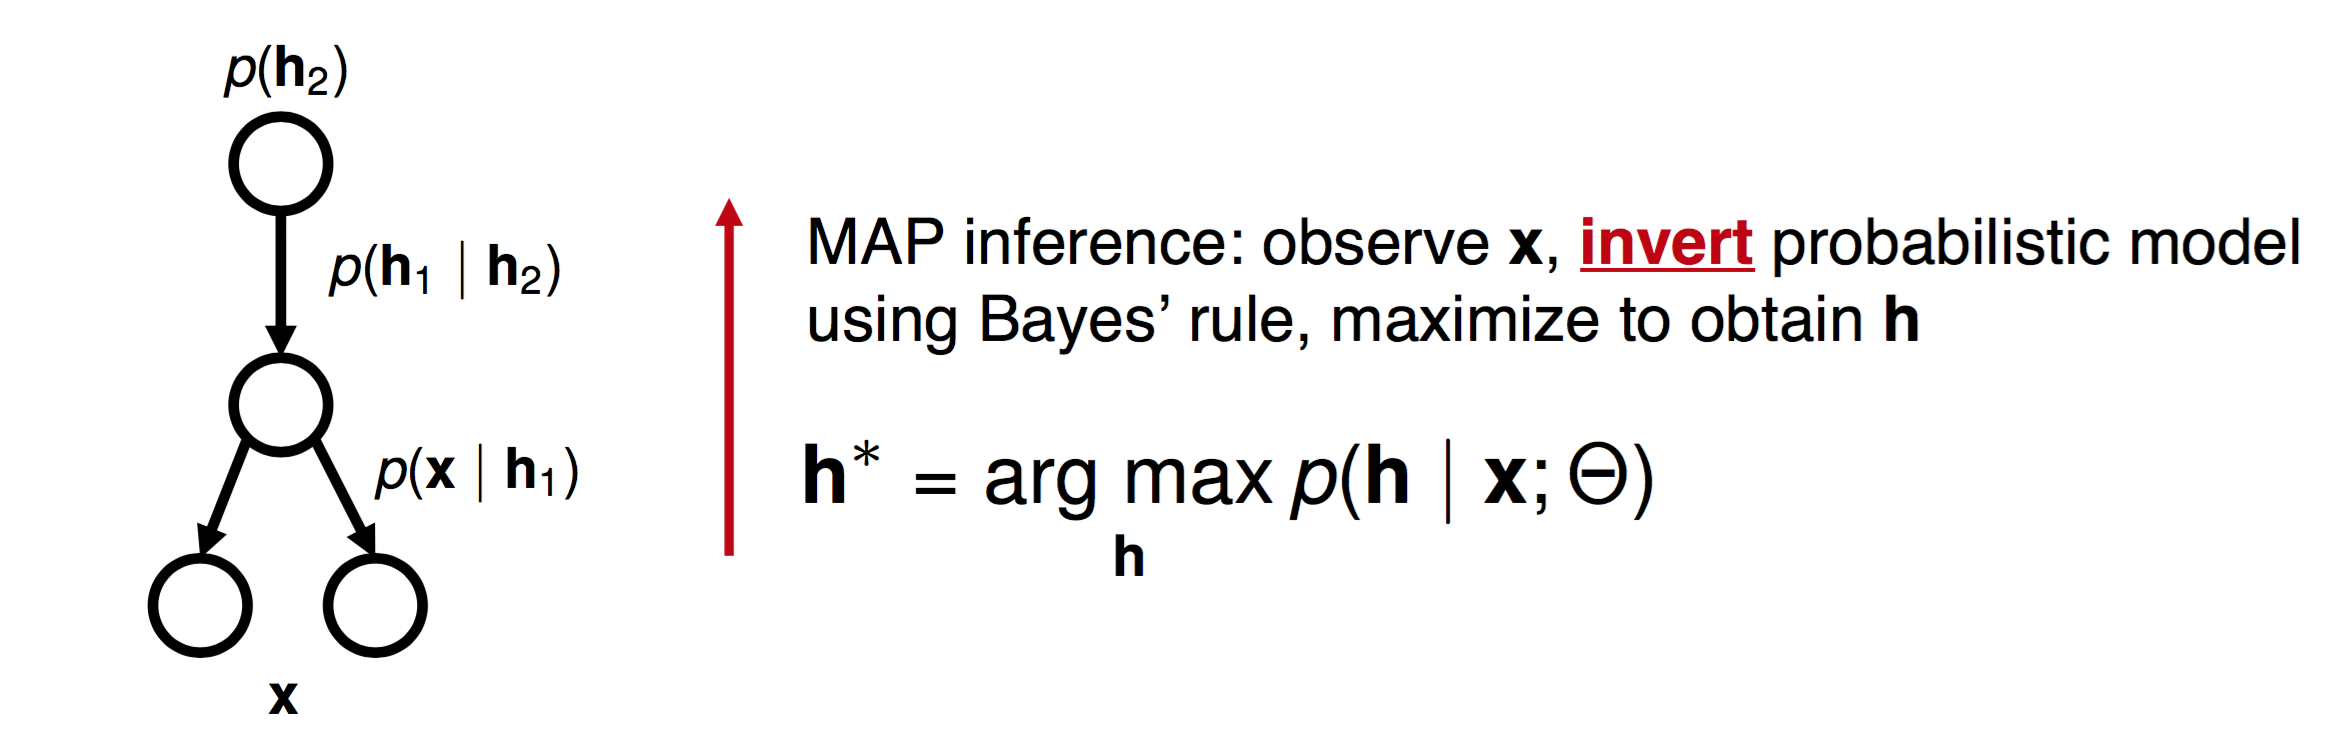
\includegraphics[width=0.9\linewidth]{06_PredictionErrorsDuringPerceptionAndLearning/figures/hierarchical_MAP.png}
            	\caption{Inference in the hierarchical generative model} 
            	\label{fig:HGM_inference}
        \end{figure}
            
\end{enumerate}

\paragraph{Inference as an optimization problem}
As we use MAP criterion to find an optimal $\bm{h}$, inference has again boiled down to solving an optimization (specifically a maximization) problem. Since the posterior probability $p(\bm{h}|\bm{x})$ is equal to the joint density $p(\bm{h},\bm{x})$ divided by $p(\bm{x})$, and we are optimizing with respect to $\bm{h}$, we can drop the denominator as follows:
\begin{equation}
    \begin{split}
        \bm{h}^* &= \argmax_h p(\bm{h}|\bm{x};\Theta)\\
        &= \argmax_h p(\bm{x},\bm{h})\\

    \end{split}
\end{equation}
Given our model assumptions listed previously and  eq.\ref{eq:joint_density}, it would be easier to deal with the log of the density. We can then revisit our optimization problem, and turn it into minimization for use of the efficiency of gradient descent: 

\begin{equation}
    \begin{split}
        \bm{h}^* &= \argmax_h p(\bm{h}|\bm{x};\Theta)\\
                &= \argmax_h p(\bm{x},\bm{h})\\
                &= \argmin_h [-\log p(\bm{x},\bm{h})]\\
    \end{split}
    \label{eq:MAP_latent}
\end{equation}
The quantity we are looking to minimize is referred to as \textbf{energy} of the dynamic system.

\paragraph{MAP estimation using gradient descent}
As we have seen in the precious chapter, we can solve eq.\ref{eq:MAP_latent} for the optimal latent variable $\bm{h}^*$ using gradient descent. Using a continuous time formulation:
\begin{equation}
    \tau \frac{d}{dt}\bm{h_i} = - \frac{\partial E(\bm{h},\bm{x},\Theta)}{\partial \bm{h_i}}
\end{equation}
where t is the time step of the gradient descent.
Next, let us plug the definition of our model, compute derivatives by hand (this can also be obtained with the help of an symbolic differentiation tool) and get:

\hl{insert equation for gradient descent for layer N, 0, and any middle layer i. I think the exact derivation of these equations are not important, it's just the idea of solving MAP estimation using gd that matters}
\begin{equation}

\label{eq:gd_latent}
\end{equation}


\subsubsection{Quick Interim Summary}
Now, let us recap what we have done so far:
\begin{itemize}
    \item We specified how a collection of random variables depend on each other using a special type of probabilistic model, the “deep nonlinear Gaussian belief network”.
    \item We decided to not be fully Bayesian, and do inference (i.e., determine latent variables when observing visible variables) using MAP estimation.
    \item We decided to use gradient descent to perform MAP estimation
    \item Remember that so far we have no neurons or neural networks
\end{itemize}

\subsubsection{What did we gain?}
From the gradient descent equation ended with an equation to solve to get the optimal latent variables. A close look into the different parts if this equation, eq.\ref{eq:gd_latent}, we can notice that it is composed of two parts. For any given layer $i$, we have
\begin{itemize}
    \item A first part with an input coming from layer $i+1$ to layer $i$
    \item A second part with an input coming from a previous layer $i-1$ to layer $i$
\end{itemize}
\begin{figure}[H]
        \centering
        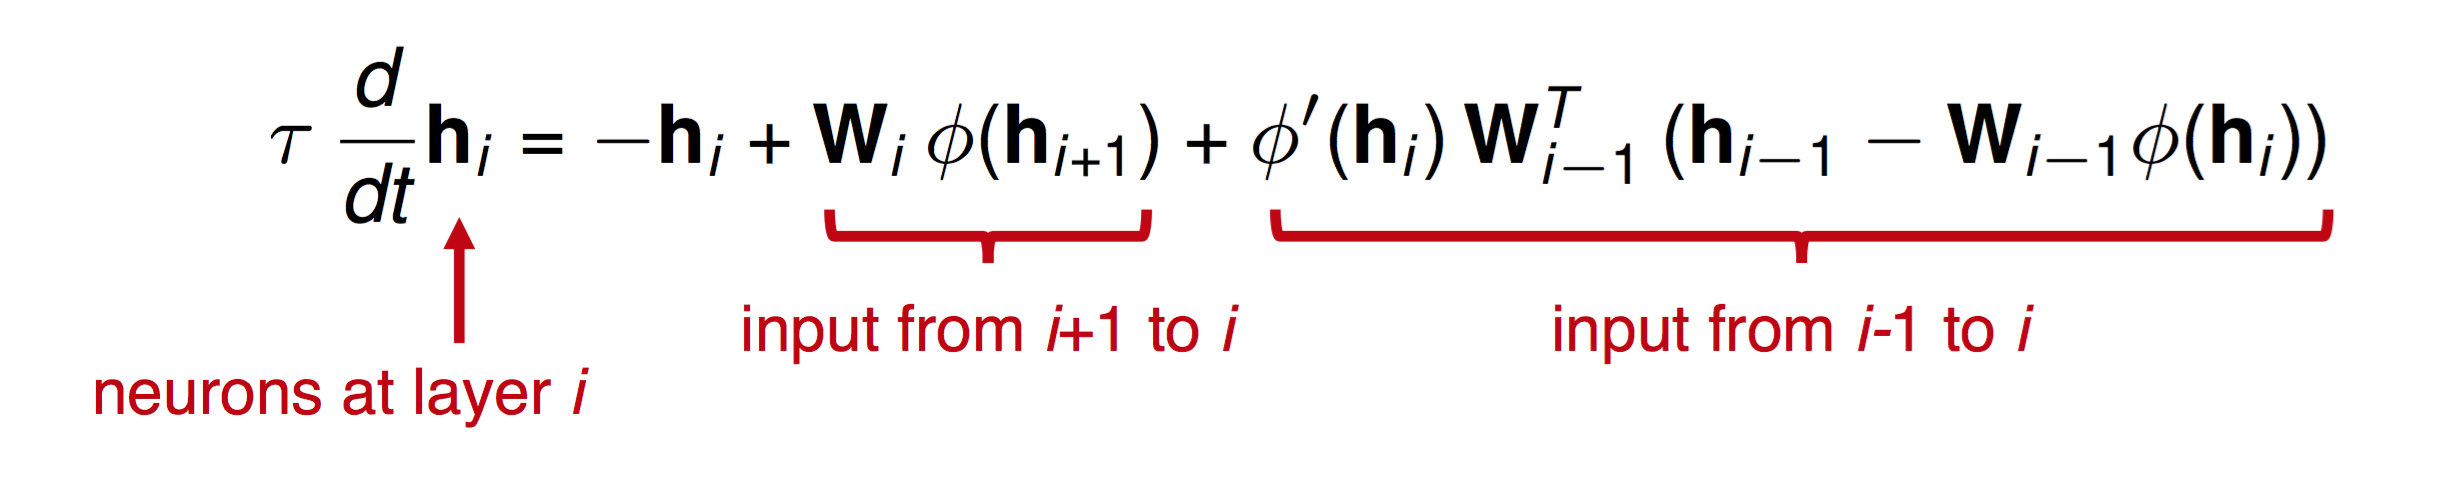
\includegraphics[width=0.9\linewidth]{06_PredictionErrorsDuringPerceptionAndLearning/figures/gd_equation.png}
        \label{fig:gd_equation_parts}
\end{figure}

\paragraph{What does it mean?} This means that for inference, we rely on previous and later layers. In other words, the neural network is in fact \textbf{recurrent} rather than an \textbf{acyclic directed graphical model} (all arrows ).

\begin{figure}[H]
        \centering
        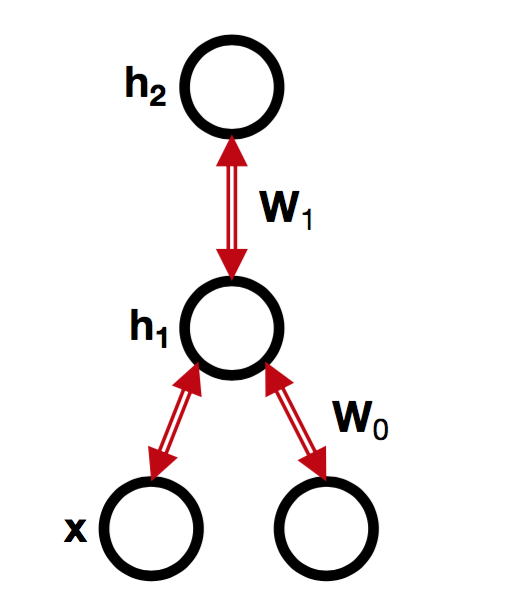
\includegraphics[width=0.4\linewidth]{06_PredictionErrorsDuringPerceptionAndLearning/figures/inference_rnn.png}
\end{figure}


Solving the system eq.\ref{eq:gd_latent} for optimality, i.e setting the derivative to zero, we get
\begin{equation}
    \bm{h}^* = \bm{W_i} \phi (\bm{h_{i+1}}^*) + \phi^\prime (\bm{h_{i}}^*)\bm{W_{i-1}}^T (\bm{h_{i-1}}^* - \bm{W_{i-1}}\phi (\bm{h_{i}}^*))
\end{equation}

\noindent With a closer look into this equation, we note that the first term corresponds to top-down \textbf{prediction}, while the second is a bottom-up \textbf{prediction error}.
\begin{figure}[H]
        \centering
        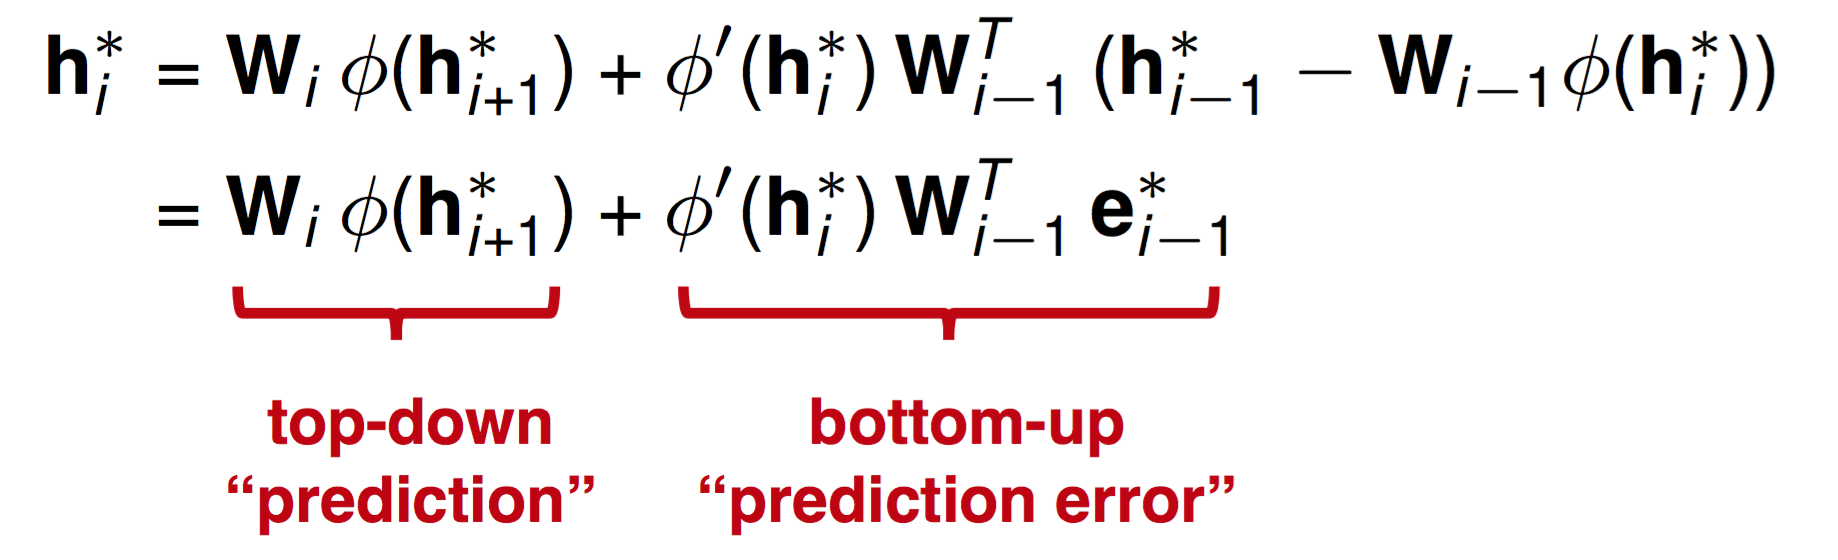
\includegraphics[width=0.9\linewidth]{06_PredictionErrorsDuringPerceptionAndLearning/figures/optimal_latent_error.png}
        \label{fig:prediction_error}
\end{figure}

\noindent Solving the recursive equation yields the following:
\begin{equation}
\begin{split}
   &\bm{e_0^*} = \bm{x} - \bm{W_0} \; \phi(\bm{h_1}^*)\\
   &\bm{e_i^*} = \phi (\bm{h_i}) \; \bm{W_{i-1}}^T \; \bm{e_{i-1}}^*
\end{split}
\end{equation}
where $0\gt< i < N$\\ 


\fbox{%
    \parbox{\textwidth}{%
We can immediately see the similarity with backpropagation. However note that here:
\begin{itemize}
    \item Errors go \textbf{forward}. They are propagated starting from the input to the top most layer N.
    \item Predictions and prediction errors are \textbf{summed up}. In contrast in backprop, we go\textbf{ forward first}, \textbf{then} propagate the errors backward.
    \item We obtained a neural dynamics which yields \textbf{at the fixed point } (steady-state) both predictions and prediction errors. In other words, both predictions and predictions errors are necessary for learning!
    \item \textbf{We are using error propagation when computing predictions}! \hl{to clarify!}
\end{itemize}}}

\subsubsection{Unsupervosed Learning}
To make inference in the previous section, we assumed the parameters $\Theta$ to be fixed. However, in fact, we would like to let our data specify them, i.e learn them from the data D. In this context, since we have no targets, this is an unsupervised learning problem.
\subsection{Dynamics for error propagation}
\end{document}